\section{Efectuarea lucrarii de laborator}
a)Pentru a realiza prima parte a sarcinii am utlizat componentele Tbutton,Tedit,Tlabel si Radiobutton:\\
\begin{center}
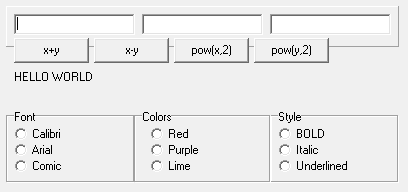
\includegraphics[scale=1]{images/A}
\end{center}
Pentru a implementa butonul x+y am poziționat în mod grafic butonul în poziția dorită ,după aceasta am
scris o funcție în limbajul C++ pentru acest buton pentru a realiza adunarea a două numere.În primele
două componente Tedit introducem numerele dorite și acționînd butonul x+y în ultima compnentă Tedit
primim rezultatul.La fel și pentru celelalte componente Tbutton.\\
\begin{center}
\lstinputlisting{source/1.cpp}
\end{center}
Pentru Tlabel cu Caption HELLO WORLD am implementat o serie de Tradiobutton grupate în GroupBox
cu denumirea respectivă pentru anumite acțiuni asupra textului.
De exemplu pentru schimbare fontului :\\
\begin{center}
\lstinputlisting{source/2.cpp}
\end{center}
b)Pentru realizarea părții a doua din lucrare de laborator am utlizat două Ttimer :unul pentru Counter și
altul pentru Timpul și Data locală din sistem:\\
\begin{center}
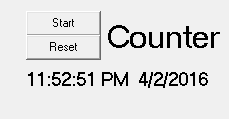
\includegraphics[scale=1]{images/B}
\end{center}
Codul pentru Timerul care afișează Timpul și Data:\\
\begin{center}
\lstinputlisting{source/3.cpp}
\end{center}
c)În a treia parte a laboratorului am utlizat TpaintBox pentru a desena un Bargraf și Diagrama:\\
\begin{center}
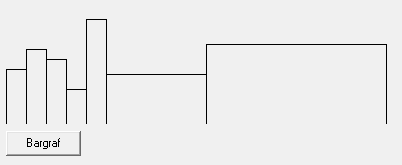
\includegraphics[scale=1]{images/C_1}\\
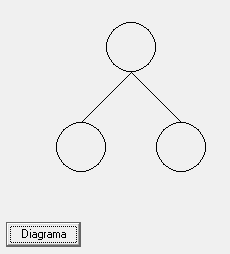
\includegraphics[scale=1]{images/C_2}\\
\end{center}
\textsc{\large Listingul Programuli}\\
\lstinputlisting{source/Unit1.cpp}

\subsection{Linkul la repozitoriul Github}
\begin{center}
\url{https://github.com/MihaiCapra/MIDPS/tree/master/MIDPS_1}
\end{center}

\subsection{Imagini}

Combinarea tuturor sarcinilor propuse intr-o singura fereastra:\\
\begin{center}
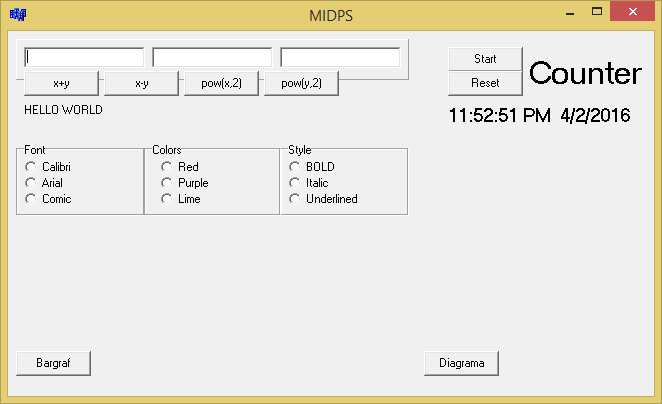
\includegraphics[scale=1]{images/main}
\end{center}

\clearpage